\documentclass[a4paper,12pt]{article}
\usepackage{amssymb} % needed for math
\usepackage{amsmath} % needed for math
\usepackage[utf8]{inputenc} % this is needed for german umlauts
\usepackage[english]{babel} % this is needed for german umlauts
\usepackage[T1]{fontenc}    % this is needed for correct output of umlauts in pdf
\usepackage[margin=2.5cm]{geometry} %layout
\usepackage{listings} % needed for the inclusion of source code
\usepackage{subcaption}
\usepackage{hyperref}
% the following is needed for syntax highlighting
\usepackage{color}

\definecolor{dkgreen}{rgb}{0,0.6,0}
\definecolor{gray}{rgb}{0.5,0.5,0.5}
\definecolor{mauve}{rgb}{0.58,0,0.82}

\lstset{ %
  language=Java,                  % the language of the code
  basicstyle=\footnotesize,       % the size of the fonts that are used for the code
  numbers=left,                   % where to put the line-numbers
  numberstyle=\tiny\color{gray},  % the style that is used for the line-numbers
  stepnumber=1,                   % the step between two line-numbers. If it's 1, each line
                                  % will be numbered
  numbersep=5pt,                  % how far the line-numbers are from the code
  backgroundcolor=\color{white},  % choose the background color. You must add \usepackage{color}
  showspaces=false,               % show spaces adding particular underscores
  showstringspaces=false,         % underline spaces within strings
  showtabs=false,                 % show tabs within strings adding particular underscores
  frame=single,                   % adds a frame around the code
  rulecolor=\color{black},        % if not set, the frame-color may be changed on line-breaks within not-black text (e.g. commens (green here))
  tabsize=4,                      % sets default tabsize to 2 spaces
  captionpos=b,                   % sets the caption-position to bottom
  breaklines=true,                % sets automatic line breaking
  breakatwhitespace=false,        % sets if automatic breaks should only happen at whitespace
  title=\lstname,                 % show the filename of files included with \lstinputlisting;
                                  % also try caption instead of title
  keywordstyle=\color{blue},          % keyword style
  commentstyle=\color{dkgreen},       % comment style
  stringstyle=\color{mauve},         % string literal style
  escapeinside={\%*}{*)},            % if you want to add a comment within your code
  morekeywords={*,...}               % if you want to add more keywords to the set
}

% this is needed for forms and links within the text
\usepackage{hyperref}
\usepackage[toc,page]{appendix}

\usepackage{tikz}
\usepackage{pgfplots}

%%%%%%%%%%%%%%%%%%%%%%%%%%%%%%%%%%%%%%%%%%%%%%%%%%%%%%%%%%%%%%%%%%%%%%
% Variablen                                                          %
%%%%%%%%%%%%%%%%%%%%%%%%%%%%%%%%%%%%%%%%%%%%%%%%%%%%%%%%%%%%%%%%%%%%%%
\newcommand{\authorName}{Ali Asgari Khoshouyeh (Student \#24868739)}
\newcommand{\tags}{\authorName, my, tags}
\title{CPEN 502 Assignment-b: Reinforcement Learning (Look Up Table)}
\author{\authorName}
\date{\today}

%%%%%%%%%%%%%%%%%%%%%%%%%%%%%%%%%%%%%%%%%%%%%%%%%%%%%%%%%%%%%%%%%%%%%%
% PDF Meta information                                               %
%%%%%%%%%%%%%%%%%%%%%%%%%%%%%%%%%%%%%%%%%%%%%%%%%%%%%%%%%%%%%%%%%%%%%%
\hypersetup{
  pdfauthor   = {\authorName},
  pdfkeywords = {\tags},
  pdftitle    = {Reinforcement Learning (Look Up Table)}
}

%%%%%%%%%%%%%%%%%%%%%%%%%%%%%%%%%%%%%%%%%%%%%%%%%%%%%%%%%%%%%%%%%%%%%%
% THE DOCUMENT BEGINS                                                %
%%%%%%%%%%%%%%%%%%%%%%%%%%%%%%%%%%%%%%%%%%%%%%%%%%%%%%%%%%%%%%%%%%%%%%
\begin{document}

\maketitle

\section*{Team Members}
We are a team of three sharing the same code base. 
\begin{itemize}
\item Christina Sun
\item Husna Kalim
\item Ali Asgari Khoushouyeh
\end{itemize}


It is noteworthy to mention that close to the extended deadline we realized that our code is orders of magnitude slower on my teammates' machines. So we sharing the plot data too. 
\pagebreak
\section*{\emph{(4) The use of a neural network to replace the look-up table and approximate the Q-function has some disadvantages and advantages.}}
\subsection*{\emph{a) There are 3 options for the architecture of your neural network. Describe and draw all three options and state which you selected and why. (3pts)}}

\begin{figure}[ht]
  \subfloat[Action as output\label{fig:first_architecture}]{
   \begin{minipage}[c][1\width]{
      0.3\textwidth}
     \centering
      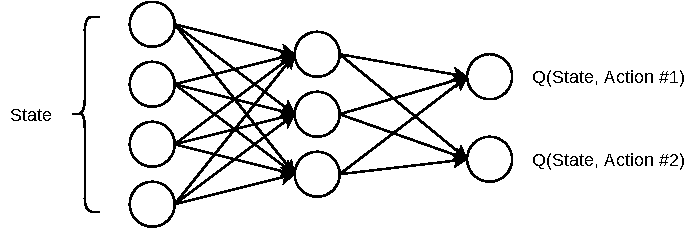
\includegraphics[width=1\textwidth]{drawio/1.pdf}
  \end{minipage}}
 \hfill  
  \subfloat[Action as input\label{fig:second_architecture}]{
   \begin{minipage}[c][1\width]{
      0.3\textwidth}
      \centering
      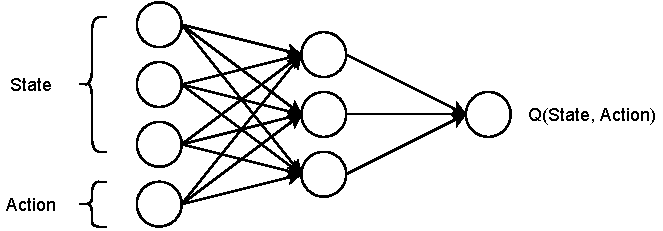
\includegraphics[width=1\textwidth]{drawio/2.pdf}
   \end{minipage}}
 \hfill  
  \subfloat[Adding time dimention\label{fig:third_architecture}]{
   \begin{minipage}[c][1\width]{
      0.3\textwidth}
      \centering
      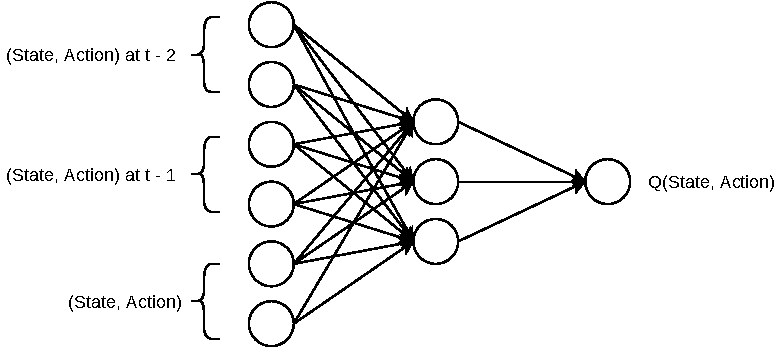
\includegraphics[width=1\textwidth]{drawio/3.pdf}
   \end{minipage}}
\caption{Different architectures considered for the neural network as the function approximator for the Q values of different game actions.}
\label{fig:architectures}
\end{figure}
FIg. \ref{fig:architectures} shows the different architectures we considered for our neural network to be plugged in instead of the lookup table. The first two architectures shown in Fig. \ref{fig:first_architecture} and Fig. \ref{fig:second_architecture} are the ones discussed in the class. The first one codes the Q value for different possible actions at each step as different neurons of the output. In the second architecture the action is coded as some input neurons and the Q value corresponding the the encoded action as the input at a certain state is coded as the single output neuron. 

The novel architecture that we used is the one shown in Fig. \ref{fig:third_architecture} which is essentially same as the second architecture, but, it also receives the state-actions of the two past time-steps as input. This is following our intuition used in the second part of the assignment where we included the past two state-actions in the lookup table keys to capture the delay of rewards as it may take some time for a bullet to hit the enemy and get reflected in the reward policy. 

\pagebreak
\subsection*{\emph{b) Show (as a graph) the results of training your neural network using the contents of the LUT from Part 2. Your answer should describe how you found the hyper-parameters which worked best for you (i.e. momentum, learning rate, number of hidden neurons). Provide graphs to backup your selection process. Compute the RMS error for your best results. (5 pts)}}

\begin{table}[hbt!]
\centering
\begin{tabular}{c|c|c|c}
Learning Rate &  Momentum &  Hidden Neurons & RMSE\\
\hline
1.00E-04 &0 & 5 & 9.666091389\\
1.00E-04& 0 &  15 &  9.660078042\\
1.00E-04 &  0 &  30 & 9.628909289\\
0.001 &  0 &  5 &  7.632740399\\
0.001 &  0 &  15 &  6.943443362\\
0.001 &  0 &  30 &  6.711401519\\
0.01 &  0 &  5 &  7.985192317\\
0.01 &  0 &  15 &  7.018144655\\
0.01 &  0 &  30 &  6.530952131\\
1.00E-04 &  0.5 &  5 &  9.148578254\\
1.00E-04 &  0.5 &  15 &  8.993952348\\
1.00E-04 &  0.5 &  30 &  9.051175005\\
0.001 &  0.5 &  5 & 7.297405961\\
0.001 &  0.5 &  15 &  \textbf{6.335407802}\\
0.001 &  0.5 &  30 &  \textbf{6.289893926}\\
0.01 &  0.5 &  5 &  7.919711744\\
0.01 &  0.5 &  15 & 7.75168296\\
0.01 &  0.5 &  30 &  8.222388904\\
1.00E-04 &  0.9 &  5 &  7.713839065\\
1.00E-04 &  0.9 &  15 & 6.790881731\\
1.00E-04 &  0.9 &  30 & 6.754064308\\
0.001 &  0.9 &  5 &  7.772037228\\
0.001 &  0.9 &  15 &  7.099569645\\
0.001 &  0.9 &  30 &  6.728784713\\
0.01 &  0.9 &  5 &    11.50926595\\
0.01 &  0.9 &  15 &  13.85358874\\
0.01 &  0.9 &  30 &  18.89859967\\

\end{tabular}
\caption{RMSE after 100 epochs under different hyper-parameter values for training the neural network on the static lookup table data.}
\label{tbl:grid_search}
\end{table}

We performed a grid search on different possible values of number of hidden neurons, momentum and learning rate. As the Q values in our lookup table ranged from $-1.2$ to several hundreds, we removed the activation of the last layer, allowing the last fully connected layer to act as a regression solver. Please note that we will keep a bipolar activation when we start training with live data, as the limited range of the output prevents the Q values to go beyond the range. 

The results are shown in Table \ref{tbl:grid_search}. As the difference between 15 hidden neurons and 30 hidden neurons (shown bold in the table) is negligible, we keep 15 neurons as it is much faster. 

\begin{figure}[hbt!]
\begin{tikzpicture}
    \begin{axis}[
        xlabel=epochs,
	 height = 10cm,
        width=\textwidth,
        ylabel=RMSE,
	 ymin=0,
        xticklabel style={rotate=30},       
	 xlabel style={yshift = -20pt}
]
    \addplot[smooth,mark=.,blue] table {static_lut.dat};
    \addlegendentry{Momentum = 0.5, Learning Rate = 0.5, Hidden Neurons  = 15}
    \end{axis}
    \end{tikzpicture}
\caption{The convergence of the select hyper-parameters over static lookup table data.}
\label{fig:static_lut}
\end{figure}

We show the convergance of the selected settings in Fig. \ref{fig:static_lut}. It shows that our neural network is able to reduce the error fitting on the lookup table static data by decreasing the error from more than 6 to around \textbf{4}. 

\pagebreak

\subsection*{\emph{c) Comment on why theoretically a neural network (or any other approach to Q-function approximation) would not necessarily need the same level of state space reduction as a look up table. (2 pts)}}
As an example, we are using the distance to the enemy as one of the dimensions of the states. When using a lookup table, it matters to decrease the number of possible values to few, so the number of entries in the lookup table do not blow up and the get revisited often. But as the neural network treats the input as a real number and does not do exact-match like the lookup table, close values also let the states be somehow recalled by the neural network. Thus, using the large number of possible values for the distant to enemy is still tractable by the neural network. That said, it is still important to limit the range of that value to something close to the other inputs so the weight initialization would fit this dimension like the other dimensions. 

\pagebreak
\section*{\emph{(5) Hopefully you were able to train your robot to find at least one movement pattern that results in defeat of your chosen enemy tank, most of the time.}}

\subsection*{\emph{a) Identify two metrics and use them to measure the performance of your robot with online training. I.e. during battle. Describe how the results were obtained, particularly with regard to exploration? Your answer should provide graphs to support your results. (5 pts)}}

\begin{figure}[hbt!]
\begin{tikzpicture}
    \begin{axis}[
        xlabel=rounds,
	 height = 10cm,
        width=\textwidth,
        ylabel=Win rate,
	 ymin=0,
        xticklabel style={rotate=30},       
	 xlabel style={yshift = -20pt},
	legend pos=north west,
]
    \addplot[smooth,mark=.,blue] table [x index=0, y index=1] {robot.NNTNinetyRobotw1g9.tex};
    \addlegendentry{$\gamma=0.9$, $n=1$}
    \end{axis}
    \end{tikzpicture}
\caption{Win rate with regard to number of training rounds.}
\label{fig:win_rate_w1g9}

\end{figure}

\begin{figure}[hbt!]
\begin{tikzpicture}
    \begin{axis}[
        xlabel=rounds,
	 height = 10cm,
        width=\textwidth,
        ylabel=Average enemy energy,
	 ymin=0,
        xticklabel style={rotate=30},       
	 xlabel style={yshift = -20pt},
	legend pos=north east,
]
    \addplot[smooth,mark=.,blue] table [x index=0, y index=3] {robot.NNTNinetyRobotw1g9.tex};
    \addlegendentry{$\gamma=0.9$, $n=1$}
    \end{axis}
    \end{tikzpicture}
\caption{Average enemy energy with regard to number of training rounds.}
\label{fig:energy_w1g9}
\end{figure}

We measure the following metrics:

\begin{enumerate}
\item \textbf{Win rate}: The number of rounds won among 100 rounds. 
\item \textbf{Average enemy energy}: The average enemy energy at the end of rounds for the course of 100 test rounds. Lower values show a better agent in causing damage to the enemy. This also will reflect our policy which only rewards on decrease in enemy energy. 

\end{enumerate}

We interleave battles of training with a robot with $\epsilon = 0.8$ and test battles of 100 rounds with a robot with $\epsilon$ set to 0.05. We only report the metrics for the test robot (i.e. $\epsilon$ set to 0.05). 

We realized that the learning process is a lot quicker if we remove the enemy distance from the input dimensions. This makes sense about our opponent which is the Corners robot. The Corners robot navigates to one corner and then tries to hit us. The best strategy that our robot comes up with is to fire so often, and this strategy is independent of the distance to enemy. Thus, we are reporting the results with that simplification hereafter. 


Fig. \ref{fig:win_rate_w1g9} shows that how the win rate for our robot increases after rounds of training. We observe a somehow abrupt  increase in the win rate. My hypothesis explaining the reason this happens is that with the neural network the Q values change gradually towards the optimal values. The optimal actions are competing the other actions with such moving Q values. Probably, because of the fact that weights are shared for different state-actions, the optimal actions exceed the Q value of the other actions and win the competition in a short number of rounds. That said, they were shifting towards the competing actions since the beginning and exceed the Q value of other actions only after 1200 rounds. 

As for the second metric, Fig. \ref{fig:energy_w1g9} shows that the average energy of the enemy decays as our agent learns more. 

\pagebreak

\subsection*{\emph{b) The discount factor $\gamma$ can be used to modify influence of future reward. Measure the performance of your robot for different values of $\gamma$ and plot your results. Would you expect higher or lower values to be better and why? (3 pts)}}

\begin{figure}[hbt!]
\begin{tikzpicture}
    \begin{axis}[
        xlabel=rounds,
	 height = 10cm,
        width=\textwidth,
        ylabel=Win rate,
	 ymin=0,
        xticklabel style={rotate=30},       
	 xlabel style={yshift = -20pt},
	legend pos=north west,
]
    \addplot[smooth,mark=.,blue] table [x index=0, y index=1] {robot.NNTNinetyRobotw10g9.tex};
    \addlegendentry{$\gamma=0.9$, $n=10$}
    \addplot[smooth,mark=.,red] table [x index=0, y index=1] {robot.NNTNinetyRobotw10g5.tex};
    \addlegendentry{$\gamma=0.5$, $n=10$}
    \addplot[smooth,mark=.,green] table [x index=0, y index=1] {robot.NNTNinetyRobotw10g1.tex};
    \addlegendentry{$\gamma=0.1$, $n=10$}
    \end{axis}
    \end{tikzpicture}
\caption{Win rate with regard to number of training rounds, under different $\gamma$.}
\label{fig:win_rate_gamma}

\end{figure}
Fig. \ref{fig:win_rate_gamma} shows the convergence of win rate for different gamma values. As can be observed the trend is similar for $\gamma = 0.1$ and $\gamma = 0.9$, but, the training seems to be more complex and converging at a less win rate for $\gamma = 0.5$. My hypothesis to explain this is that high gamma values will lead to quicker convergence in the Q-learning side, meaning rewards propagate quicker to the earlier stages. With the low gamma values the Q values used to update the neural network change slower, so the neural network has more time to adapt. But the intermediate gamma value (0.5) has none of the advantages. It is neither slow while providing updates to the neural network, nor needing less steps in the convergence of Q values, thus it leads to a less ultimate effectiveness of training. 

Intuitively, there are two dynamical systems interacting with each other and trying to converge here, one is the neural network, the other is the Q-learning values. These two are chained together. High gamma values help the Q-learning and low gamma values help the neural network. But the intermediate value does not provide any of the advantages. 

\pagebreak
\subsection*{\emph{c) Theory question: With a look-up table, the TD learning algorithm is proven to converge – i.e. will arrive at a stable set of Q-values for all visited states. This is not so when the Q-function is approximated. Explain this convergence in terms of the Bellman equation and also why when using approximation, convergence is no longer guaranteed. (3 pts)}}

If you unroll the Q-value based on the Q-learning formula, assuming the reward is some stochastic random variable, we can define the Q-value as the following expected:

$$V(s) = E[r_0 + \gamma V(s_1) | s_0 = s]$$

so $r_0 + \gamma V(s_1)$ is an unbiased estimate for the random variable $V(s)$ \footnote{\url{https://en.wikipedia.org/wiki/Temporal\_difference\_learning\#Mathematical\_formulation}}. This means initializing $V$ with arbitrary values for states and then sampling the consequent states of the game ($s$ and $s'$), and updating the values based on the following rule with a positive learning rate ($\alpha$) will converge to the unbiased estimates:

$$V(s) \leftarrow V(s) + \alpha (r + \gamma V(s') - V(s))$$


Unfortunately, with using a function approximation this update rule is not done precisely, instead the left-hand-side shifts closer to the right-hand-side, while implicitly corrupting values for other states, thus this update rule which is guaranteed to converge on the unbiased estimates is not performed and the guarantee does not hold. 

\pagebreak

\subsection*{\emph{d) When using a neural network for supervised learning, performance of training is typically measured by computing a total error over the training set. When using the NN for online learning of the Q-function in robocode this is not possible since there is no a-priori training set to work with. Suggest how you might monitor learning performance of the neural net now. (3 pts)}}

\begin{figure}[hbt!]
\begin{tikzpicture}
    \begin{axis}[
        xlabel=rounds,
	 height = 10cm,
        width=\textwidth,
        ylabel=MSE,
	 ymin=0,
        xticklabel style={rotate=30},       
	 xlabel style={yshift = -20pt}
]
    \addplot[smooth,mark=.,blue] table [x index=0, y index=4] {robot.NNTNinetyRobotw20g9.tex};
    \addlegendentry{$\gamma=0.9$, $n=20$}
    \end{axis}
    \end{tikzpicture}
\caption{MSE over 20 subsequent states, with regard to rounds of training.}
\label{fig:nn_metric}
\end{figure}

Inspired by the idea of replay memory, we use the loss over a local window of data points. Fig. \ref{fig:nn_metric} shows how the MSE as a metric for the performance of the neural network decreases after rounds of training. With the use of replay memory we are able to calculate this loss over 20 subsequent data points.

\pagebreak
\subsection*{\emph{e) At each time step, the neural net in your robot performs a back propagation using a single training vector provided by the RL agent. Modify your code so that it keeps an array of the last say n training vectors and at each time step performs n back propagations. Using graphs compare the performance of your robot for different values of n. (4 pts)}}

\begin{figure}[hbt!]
\begin{tikzpicture}
    \begin{axis}[
        xlabel=rounds,
	 height = 10cm,
        width=\textwidth,
        ylabel=Win rate,
	 ymin=0,
        xticklabel style={rotate=30},       
	 xlabel style={yshift = -20pt},
	legend pos=north west,
]
    \addplot[smooth,mark=.,red] table [x index=0, y index=1] {robot.NNTNinetyRobotw10g5.tex};
    \addlegendentry{$\gamma=0.9$, $n=10$}
    \addplot[smooth,mark=.,green] table [x index=0, y index=1] {robot.NNTNinetyRobotw20g9.tex};
    \addlegendentry{$\gamma=0.9$, $n=20$}
    \end{axis}
    \end{tikzpicture}
\caption{Win rate with regard to number of training rounds, under different $\gamma$.}
\label{fig:win_rate_n}
\end{figure}

Fig. \ref{fig:win_rate_n} shows the different convergence behaviour with regard to different values for the window size of the replay memory. We observe that high value for the window size leads to a better win rate eventually. My hypothesis to explain this is that a larger local window allows the neural network to skip local optima and hopefully take better strategies. 

\pagebreak
\section*{\emph{(6) Overall Conclusions}}
\subsection*{\emph{a) This question is open-ended and offers you an opportunity to reflect on what you have learned overall through this project. For example, what insights are you able to offer with regard to the practical issues surrounding the application of RL \& BP to your problem? E.g. What could you do to improve the performance of your robot? How would you suggest convergence problems be addressed? What advice would you give when applying RL with neural network based function approximation to other practical applications? (4 pts)}}

Here are some insights we came up with: 
\begin{enumerate}
\item More hidden neurons make the neural network to be able to learn more complex patterns. We were able to achieve less numerical error over our static lookup table data with more number of hidden neurons.

\item In a game where there are delays for the rewards to get effective (e.g. for firing to result in change in enemy energy) one trick to turn the environment back to a Markov environment is to treat series of subsequent states as some macro states which are path independent and actually form a Markov chain. 

\item A lot of the time it is possible that large learning rates result in lack of convergence of the neural network. The search for a working and yet efficient learning rate has a rule of thumb of searching with different orders of magnitude and it is not required to search with linear steps. 

\item To approach a complex implementation such as Q-learning with a deep neural network, it is always better to first break it into sub-problems. We have done this several times during the project. To test our Q-learning code we used a simpler game with the goal of navigating the robot the top right corner of the game only. To debug our neural network we started with a single layer wide neural network which was quite imitating a lookup table. To check if our neural network is capable of learning the game patterns we were instructed to first train the neural network over the static data from a lookup table. 

\end{enumerate}

\pagebreak
\subsection*{\emph{b) Theory question: Imagine a closed-loop control system for automatically delivering anesthetic to a patient under going surgery. You intend to train the controller using the approach used in this project. Discuss any concerns with this and identify one potential variation that could alleviate those concerns. (3 pts)}}

The essential problem here is that there is no grant for killing the patient because of the RL algorithm performing trial and errors. 

To fix this, I would suggest training the control system on a pseudo patient which only measures the dosage of anaesthetic over time. 

To further make things safe, after the training is done we can try applying formal verification to ensure no harmful state is met while the execution of the trained agent. 

We can also put safeguards in the controller, such as maximum limits of the dosage so that it does not pass the safe limits. 

\pagebreak
\begin{appendices}
\section{Source Codes}
    \lstinputlisting[language=Java,caption=autograd/Addition.java]{../src/main/java/autograd/Addition.java}
\lstinputlisting[language=Java,caption=autograd/Exponentiation.java]{../src/main/java/autograd/Exponentiation.java}
\lstinputlisting[language=Java,caption=autograd/IInitializer.java]{../src/main/java/autograd/IInitializer.java}
\lstinputlisting[language=Java,caption=autograd/IOperator.java]{../src/main/java/autograd/IOperator.java}
\lstinputlisting[language=Java,caption=autograd/IVariable.java]{../src/main/java/autograd/IVariable.java}
\lstinputlisting[language=Java,caption=autograd/Multiplication.java]{../src/main/java/autograd/Multiplication.java}
\lstinputlisting[language=Java,caption=autograd/Negation.java]{../src/main/java/autograd/Negation.java}
\lstinputlisting[language=Java,caption=autograd/Operation.java]{../src/main/java/autograd/Operation.java}
\lstinputlisting[language=Java,caption=autograd/Operator.java]{../src/main/java/autograd/Operator.java}
\lstinputlisting[language=Java,caption=autograd/Parameter.java]{../src/main/java/autograd/Parameter.java}
\lstinputlisting[language=Java,caption=autograd/Sigmoid.java]{../src/main/java/autograd/Sigmoid.java}
\lstinputlisting[language=Java,caption=autograd/UniformInitializer.java]{../src/main/java/autograd/UniformInitializer.java}
\lstinputlisting[language=Java,caption=dataset/BinaryToBipolarWrapper.java]{../src/main/java/dataset/BinaryToBipolarWrapper.java}
\lstinputlisting[language=Java,caption=dataset/DataPoint.java]{../src/main/java/dataset/DataPoint.java}
\lstinputlisting[language=Java,caption=dataset/IDataSet.java]{../src/main/java/dataset/IDataSet.java}
\lstinputlisting[language=Java,caption=dataset/XORBinaryDataSet.java]{../src/main/java/dataset/XORBinaryDataSet.java}
\lstinputlisting[language=Java,caption=nn/BipolarSigmoid.java]{../src/main/java/nn/BipolarSigmoid.java}
\lstinputlisting[language=Java,caption=nn/ConvergenceCollector.java]{../src/main/java/nn/ConvergenceCollector.java}
\lstinputlisting[language=Java,caption=nn/Factory.java]{../src/main/java/nn/Factory.java}
\lstinputlisting[language=Java,caption=nn/IFitCallback.java]{../src/main/java/nn/IFitCallback.java}
\lstinputlisting[language=Java,caption=nn/ILayer.java]{../src/main/java/nn/ILayer.java}
\lstinputlisting[language=Java,caption=nn/Linear.java]{../src/main/java/nn/Linear.java}
\lstinputlisting[language=Java,caption=nn/MinimumSquaredError.java]{../src/main/java/nn/MinimumSquaredError.java}
\lstinputlisting[language=Java,caption=nn/Model.java]{../src/main/java/nn/Model.java}
\lstinputlisting[language=Java,caption=nn/Sigmoid.java]{../src/main/java/nn/Sigmoid.java}
\lstinputlisting[language=Java,caption=optimization/GradientDescent.java]{../src/main/java/optimization/GradientDescent.java}
\lstinputlisting[language=Java,caption=optimization/ILoss.java]{../src/main/java/optimization/ILoss.java}
\lstinputlisting[language=Java,caption=optimization/IOptimizer.java]{../src/main/java/optimization/IOptimizer.java}
\lstinputlisting[language=Java,caption=autograd/VariableTest.java]{../src/test/java/autograd/VariableTest.java}
\lstinputlisting[language=Java,caption=nn/NeuralNetworkTest.java]{../src/test/java/nn/NeuralNetworkTest.java}
\lstinputlisting[language=Java,caption=optimization/GradientDescentTest.java]{../src/test/java/optimization/GradientDescentTest.java}

\end{appendices}

\end{document}
